\documentclass[10pt]{beamer}
\usepackage{graphicx}
\usepackage{amsmath}
\usepackage{bibentry}
\usepackage{biblatex}
\usepackage{multirow}
\usepackage{adjustbox}
\usepackage[font=scriptsize]{caption}
\usepackage{subcaption}
\usepackage{hyperref}
\usepackage[ruled]{algorithm2e}
\usepackage{algorithmic,float}
\usepackage{dirtytalk}
\usepackage{marginnote}
\usepackage{tikz}
\usepackage[T1]{fontenc}
\usepackage{transparent}
\usepackage{eso-pic}
\usepackage{lipsum}
\usepackage{xcolor}
\usepackage{wrapfig}

\SetKwInOut{Parameter}{parameter}

\captionsetup[figure]{labelsep=period}
\captionsetup[subfigure]{labelformat=simple}
\renewcommand\thesubfigure{\thefigure.\alph{subfigure}.}


\setbeamertemplate{navigation symbols}{}
\setbeamertemplate{caption}[number]
\bibliography{Bibliography}

\graphicspath{{/Users/flavioforenza/Desktop/latex/images/}}
\setbeamertemplate{footline}[frame number]

\usetheme{Darmstadt}


%\title[short]{UNIVERSITÀ DEGLI STUDI DI MILANO}
\title[]{Distilled-Single-Shot-Detector (DSSD): un nuovo modello di guida autonoma ad alta inferenza}

\author[Flavio Forenza]{
                        
\includegraphics[scale = 0.05]{
                                        unimilogo.png}\\ 
                                        \vspace{0.1cm}
                                        \fontfamily{cmr}\selectfont {\bfseries{UNIVERSITÀ DEGLI STUDI DI MILANO}}\\
                                        \fontfamily{cmr}\selectfont \emph{Laurea magistrale in Informatica}\\
                                        \vspace{1cm}
                                        }
\date{\scriptsize Aprile 2022}


\begin{document}

\begin{frame}
    \maketitle
    \vspace{-2.5cm}
    \begin{minipage}{\linewidth}
        \centering
        \begin{minipage}{0.45\linewidth}
            \begin{flushleft}
                \emph{Relatore:}\\
                Prof. Vincenzo Piuri\\
                \emph{Correlatore:}\\
                Dott. Angelo Genovese
            \end{flushleft}
        \end{minipage}
        \begin{minipage}{0.45\linewidth}
            \begin{flushright}
                \emph{Laureando:}\\
                Flavio Forenza
            \end{flushright}
        \end{minipage}
    \end{minipage}
\end{frame}

\logo{
\includegraphics[width=0.1\linewidth]{unimilogo.png}}

\section{\centering{"Distilled-Single-Shot-Detector (DSSD): un nuovo modello di guida autonoma ad alta inferenza"}}

\begin{frame}{STATO DELL'ARTE - OBIETTIVO}
    Ricerca basata sullo sviluppo e sull'implementazione di grandi modelli deep learning in sistemi a 
    limitate risorse computazionali (es: embedded, mobile, indossabbili, etc.).\\
    Requisiti da soddisfare:\\
    \hspace{1cm}
    \begin{minipage}{\linewidth}
        \centering
        \begin{minipage}{0.45\linewidth}
            \begin{enumerate}
                \item Buona velocità di inferenza
                \item Risparmio energetico
                \item Minor occupazione della memoria
                \item Basso impatto sull'accuratezza
                \item Miglior gestione delle risorse HW/SW
            \end{enumerate}
        \end{minipage}
        \begin{minipage}{0.45\linewidth}
            \begin{figure}
                \centering
                
\includegraphics[width = \linewidth]{objective.png}
                \centering
            \end{figure}
        \end{minipage}
    \end{minipage}
\end{frame}
\begin{frame}{CRISI DEI SEMICONDUTTORI}
    
\end{frame}
\begin{frame}{LAVORO DI TESI}
    Lo studio della tesi si è concentrato sulla ricerca e sull'implementazione 
    di varie tecniche di compressione e, allo stesso tempo, di ottimizzazione, 
    in grado di offrire supporto allo sviluppo di un nuovo modello di guida autonoma efficiente e ad alta velocità di inferenza.\\
    \vspace{0.3cm}
    Quest'ultimo, deriva dallo studio di due modelli già noti allo stato dell'arte:
    \begin{minipage}{\linewidth}
        \centering
        \begin{minipage}{0.45\linewidth}
            \begin{enumerate}
                \item {\bfseries{\emph{MobileNet-V1}}}\footnotemark[1]: specializzato nel task di \emph{Image classification};
                \item {\bfseries{\emph{Single-Shot-Detector (SSD)}}}\footnotemark[2]: specializzato nel task di \emph{Object Detection}.
            \end{enumerate}
        \end{minipage}
        \begin{minipage}{0.45\linewidth}
            \begin{figure}
                \centering
                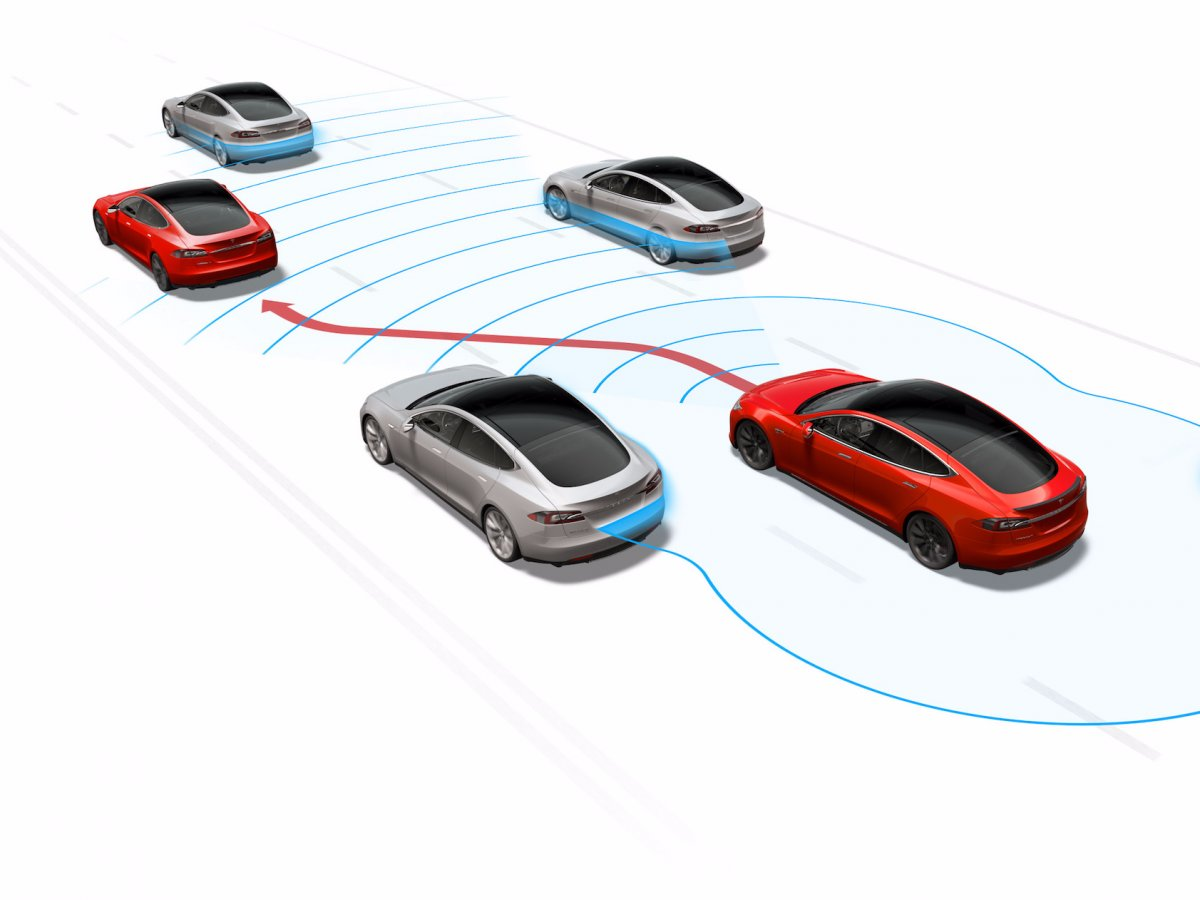
\includegraphics[width = \linewidth]{tesla_autopilot.png}
                \centering
            \end{figure}
        \end{minipage}
    \end{minipage}
    \footnotetext[1]{\emph{Andrew G. Howard et al., "MobileNets: Efficient Convolutional Neural Networks for Mobile Vision Applications", 2017.}}
    \footnotetext[2]{\emph{Liu et al., "SSD: Single Shot MultiBox Detector", 2016.}}
\end{frame}
\begin{frame}{ARCHITETTURE DI RIFERIMENTO}
    Tutti i test sono stati eseguiti su tre architetture differenti in termini di performance, dimensioni e costo.
     
    
\end{frame}

\end{document}